
\documentclass[addpoints,12pt]{exam}
\usepackage{amssymb,amsmath,amsthm,graphicx}
\usepackage{tikz}
\usepackage{listings}
\usepackage{courier}
\usepackage{graphicx}
\usepackage{scrextend}
\usepackage{adjustbox}

\lstset{frame=l,xleftmargin=\fboxsep,xrightmargin=-\fboxsep,colframe=gray}
\lstset{basicstyle=\ttfamily\footnotesize,breaklines=true}


\newcommand{\code}[1]{{\texttt{#1}}}
\newcommand{\mcode}[1]{{\text{\texttt{#1}}}}

\linespread{1.2}
\usepackage{color}
\definecolor{gray}{rgb}{0.3,0.3,0.3}



\pagestyle{headandfoot}
\runningheadrule
\firstpageheader{Math 9}{\,}{Final Exam -- version {\Huge \color{gray} \fontfamily{pbk}\selectfont A}}
\runningheader{Math 9}
              {\,}
              {Final Exam ver A, Page \thepage\ of \numpages}
\firstpagefooter{}{}{}
\runningfooter{}{}{}
\newtheorem{theorem}{Theorem}
\newtheorem{definition}{Definition}
\newtheorem{expectation}{Expectation}

\newcommand{\RR}{\mathbb{R}}

\begin{document}
\begin{center}
\fbox{\fbox{\parbox{5.5in}{\centering
{\tt Directions:} The exam is 120 minutes long. Please read each question carefully. 
\vspace{10pt}

When asked to write code, you should write working Python code that has correct syntax. You should explain in 1-2 sentences what the idea for your solution is or write next to your code what it is doing. This will increase your chances of getting full/partial credit. 

Use the backs of the pages if needed.
}}}
\end{center}


\vspace{0.2in}

\makebox[\textwidth]{Last Name:\enspace\hrulefill}

\vspace{0.2in}

\makebox[\textwidth]{First Name:\enspace\hrulefill}

\vspace{0.2in}

\makebox[\textwidth]{Student ID \#:\enspace\hrulefill}

\vspace{0.2in}

\vspace{1in}

\gradetable

\newpage

\begin{questions}

\question[20]
Write down the output of the following programs.

\begin{enumerate}
\item 
\begin{lstlisting}[language=python]
x = 1
s = 0
for i in range(8):
    s += x
    x *= 10
print(s)
\end{lstlisting}

    \vfill

\item 
\begin{lstlisting}[language=python]
def f(n):
    if n > 0:
        return n + g(n - 1)
    return 1

def g(n):
    return f(n) - n

print(f(11))
\end{lstlisting}
\vfill


\item 
\begin{lstlisting}[language=python]
xs = [0,2,7]
x = sum(map(lambda x: 2 ** x, xs))
print(x)
\end{lstlisting}
\vfill

\item 
\begin{lstlisting}[language=python]
# fin
def g(n):
    if n == 0:
        return [] 
    return [n % 2] + g(n // 2) 

print(g(133))
\end{lstlisting}
%
\vfill

\end{enumerate}

\newpage
\question[20] Produce the following lists without using for or while loops. 
\begin{enumerate}
  \item \code{[11, 101, 1001, 10001, 100001, 1000001, 10000001, 100000001, 1000000001]}
    \vfill
  \item \code{[0, 0, 1, 1, 2, 2, 3, 3, 4, 4, 5, 5, 6, 6, 7, 7, 8, 8, 9, 9]}
    \vfill
  \item \code{[0, 101, 2, 103, 4, 105, 6, 107, 8, 109, 10, 111, 12, 113, 14]}
    \vfill
    
\end{enumerate}




\newpage
\question[20] Write code that will produce the following graphs (or something that looks like it; use \code{plt.plot(X, Y)} and \code{plt.scatter(X, Y)}).
\begin{enumerate}
\item
\adjustbox{valign=t}{
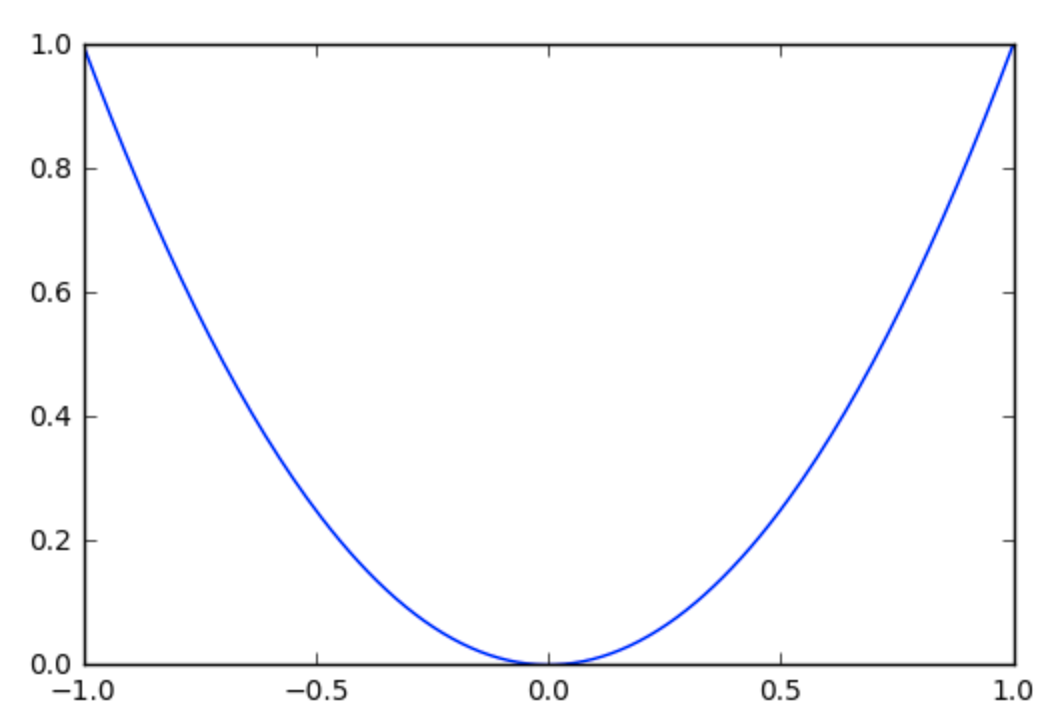
\includegraphics[valign=t, width=3.1in]{graph_quad.png}
}
\vfill
\item 
\adjustbox{valign=t}{
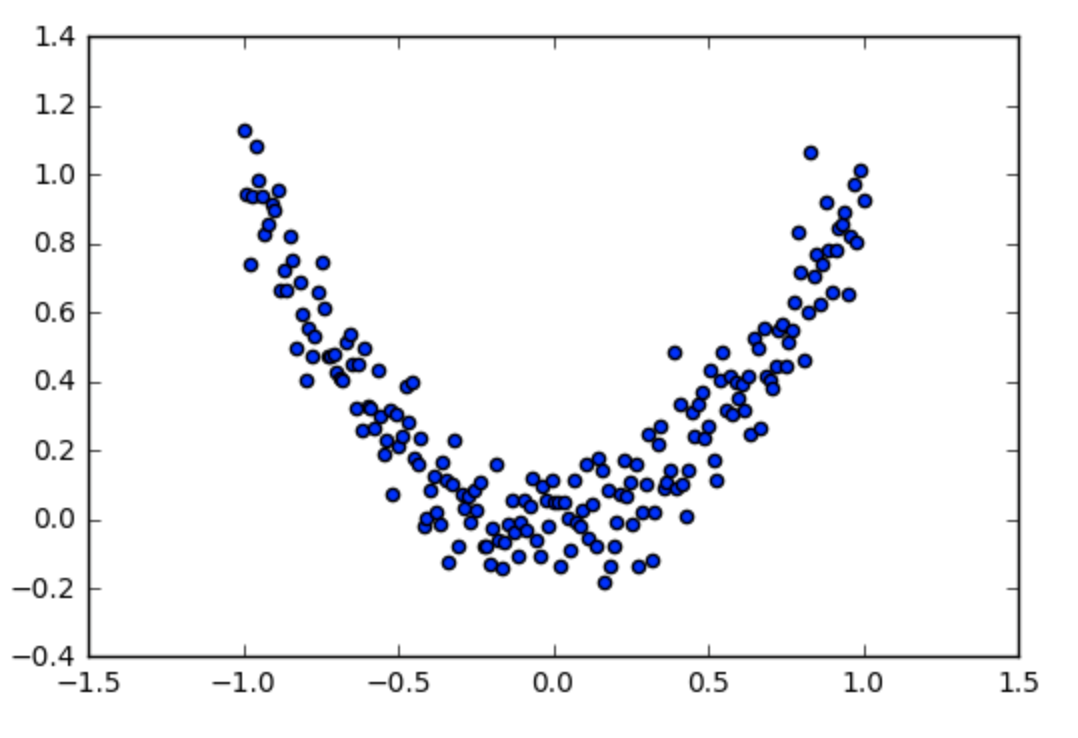
\includegraphics[valign=t, width=3.2in]{graph_noise_quad.png}
}
\vfill
\end{enumerate}





\newpage
\question[20] Complete the code below to implement the function \code{square(n)} that will return a numpy array with the numbers $1,2,\dots,n^2$ arranged in a square.

Examples:
\begin{lstlisting}[language=python]
In:   square(3)
Out:  array([[1, 2, 3],
             [4, 5, 6],
             [7, 8, 9]])


In:   square(4)
Out:  array([[ 1,  2,  3,  4],
             [ 5,  6,  7,  8],
             [ 9, 10, 11, 12],
             [13, 14, 15, 16]])
\end{lstlisting}

\begin{lstlisting}[language=python]
def square(n):
    X = 
    return 
\end{lstlisting}

\vfill

Complete the code below to implement the function \code{square\_2(n)}, which produces the same square as the above, but with all entries except the ones at the edges set to zero. 
\begin{lstlisting}[language=python]
In:   square_2(n) 
Out:  array([[ 0,  1,  2,  3,  4,  5,  6],
             [ 7,  0,  0,  0,  0,  0, 13],
             [14,  0,  0,  0,  0,  0, 20],
             [21,  0,  0,  0,  0,  0, 27],
             [28,  0,  0,  0,  0,  0, 34],
             [35,  0,  0,  0,  0,  0, 41],
             [42, 43, 44, 45, 46, 47, 48]]) 
\end{lstlisting}

\begin{lstlisting}[language=python]
def square_2(n):
    X = squa(n)
    
    
    return X
\end{lstlisting}

\vfill

\newpage
\question[20] Implement a function \code{isprime(n)} that will return \code{True} if an integer \code{n} is prime and \code{False} otherwise.  

\newpage
\question[20] Recall the \code{Polynomial} class from the homework that stores a polynomial as a list of its coefficients. Implement the \code{\_\_eval\_\_(self, x)} function that returns a new polynomial which represents the sum of the polynomials self and other.  


\begin{lstlisting}[language=python]
class Polynomial():
    def __init__(self, xs):
        self.coeffs = xs
    
    def __repr__(self):
        if self.coeffs == []:
            return "0"
        c = ""
        for i, x in enumerate(self.coeffs):
            c += str(x) + "x" + "^" + str(i) + " + "
        return c[:-3]
    
    def eval(self, x):
\end{lstlisting}

\newpage
\question[20] Write a function \code{is\_rearranged\_palindrome(n)} that takes an integer \code{n} and returns \code{True} if and only if the digits of \code{n} can be rearranged to make a palindrome. (You can assume that \code{n} has an even number of digits if it makes things easier) 


\newpage
\question[20] Your buddy Joker has given you a coin that you think might be unfair. You can flip the coin by calling the function \code{flip()} which returns either 0 or 1 (for heads or tails). You can call \code{flip()} at most $1000$ times. Write code that will compute your best estimate for the probability of \code{flip()} being tails.  


\newpage
\question (extra-credit, 20 points) Only near-perfect answers will receive the extra-credit. Please don't attempt this problem if you haven't already finished all other problems and checked your answers. 

Monty Hall Problem: You are in a game-show. The host tells you that you can choose between the three doors in front of you. Only one of the doors has a pot of gold behind it. You choose door 1. The host opens one of the other doors and shows you that it did not have the pot of gold. The host then gives you the choice to stick to your original choice of door 1 or swich your choice to the remaining other door. Should you switch? 

Write a simulation that evaluates the success rate of two strategies: 
(a) always switching to the remaining other door, 
(b) always sticking with door 1. 

\end{questions}
\end{document}
